\documentclass[a4paper, 12pt]{article}

%%%%%%%%%%%%%%%%%%% Packages

\usepackage[french, english]{babel}
\usepackage[noheader]{packages/sleek}
\usepackage{packages/sleek-title}

%%%%%%%%%%%%%%%%%%% Titlepage

\logo{resources/pdf/logo-uliege.pdf}
\institute{University of Liège}
\title{Project 2}
\subtitle{Information and coding theory}
\author{
    Maxime \textsc{Meurisse} (s161278)\\
    François \textsc{Rozet} (s161024)\\
}
\context{Master in Computer Science and Engineering}
\date{Academic year 2019-2020}

%%%%%%%%%%%%%%%%%%% Bibliography

\addbibresource{./resources/bib/references.bib}

%%%%%%%%%%%%%%%%%%% Others

\def\X{\mathcal{X}}
\def\Y{\mathcal{Y}}
\def\Z{\mathcal{Z}}

%%%%%%%%%%%%%%%%%%% Document

\begin{document}
    % ----- Title page ----- %
    
    \maketitle
    
    % ----- Source coding and reversible data compression ----- %
    
    \section*{Source coding and reversible data compression}
    
    The code relative to this section questions is presented in the file \texttt{text.py}.
    
    \begin{enumerate}[leftmargin=*]
        % Question 1
        
        \item The set of source symbols from the text sample $S$ is determined by listing the different symbols appearing in the text sample via the \texttt{unique} function of the \texttt{numpy} python library. This set contains $Q = 73$ symbols presented, in the order of the ASCII convention, in Table \ref{tab:q1.symbols}.
        
        \begin{table}[H]
            \centering
            \begin{tabular}{|c|c|c|c|c|c|c|c|c|c|c|c|c|c|c|c|c|c|c|c|}
                \hline
                \textbackslash n & & ! & " & \& & ' & , & - & . & / & 0 & 1 & 2 & 4 & 5 & 6 & 8 & 9 & : & =\\ \hline
                ? & A & B & C & D & E & F & G & H & I & J & K & L & M & N & O & P & R & S & T\\ \hline
                U & V & W & X & Y & Z & \_ & a & b & c & d & e & f & g & h & i & j & k & l & m\\ \hline
                n & o & p & q & r & s & t & u & v & w & x & y & z\\ \cline{1-13}
            \end{tabular}
            \caption{Set of source symbols of $S$.}
            \label{tab:q1.symbols}
        \end{table}
        
        % Question 2
        
        \item The marginal probability distribution of a symbol of $S$ is calculated by dividing the number of occurrences of this symbol in the text sample by the total number of symbols in the text. The marginal probabilities of each symbol are presented in Table \ref{tab:q4.symbols}.
        
        By considering only the marginal probability distribution of the symbols, two assumptions are made : (successive) symbols are independent from each other and the symbol distribution is invariant with shifts in the (time) index. In other words, it is supposed that the symbols are coded \emph{one by one} by a \emph{memoryless} \emph{stationary} source.
        
        Mathematically, for all symbol $s$
        \begin{align*}
            P(\X_{i} = s \mid \X_{i - 1}, \ldots, X_{1}) & = P(\X_{i} = s) = P(\X_1 = s) & \forall i \geq 0
        \end{align*}
        In practice, in languages, especially natural ones like English, this assumption is not true : the syntactic and semantic rules as well as the vocabulary imply that the successive symbols are \emph{dependent} from each other.
        
        % Question 3
        
        \item The requested function is named \texttt{Huffman.code} and implements the Huffman's algorithm \cite{huffman1952method}.
        
        To implement the Huffman tree, we chose to represent a node as a \emph{dictionary} whose keys are the labels of the tree \emph{branches} and the values are the \emph{sub-trees} (nodes) or leafs. The keys are selected within the coding alphabet. Finally, the leafs of the tree are the \emph{source symbols}.
        
        The first step of our implementation is to assign to each symbol $s_i$ a leaf-node. Then the leafs are inserted into a \emph{priority queue} according to their marginal probability. The priority is actually computed as the inverse of the probability so that symbols with the lowest probability have the highest priority.
        
        Then, the algorithm repeats the following procedure until there is only one element left in the queue :
        \begin{enumerate}[noitemsep, label=\roman*.]
            \item Select (pop) the \emph{two} nodes with the highest priority;
            \item Create a new sub-tree with branches (labeled with coding alphabet symbols) leading to the selected nodes;
            \item Compute the probability of the sub-tree as the sum of the probabilities of the selected nodes;
            \item Insert the sub-tree in the priority queue according to its priority (inverse of probability).
        \end{enumerate}
        
        The remaining element is a valid Huffman tree.
        
        To extend this procedure to any alphabet size, there is only to change the number of nodes that are selected and merged into a sub-tree at each iteration. Actually, our implementation can already generate a Huffman code of any alphabet size, as the latter is an argument of the function.
        
        % Question 4
        
        \item Using the previously defined function, the optimal code for the marginal distribution of source symbols is obtained and presented in Table \ref{tab:q4.symbols}.
        
        \begin{table}[H]
            \centering
            \resizebox{\textwidth}{!}{
                \begin{tabular}{c|c|c||c|c|c}
                    {\bf Symbol} & {\bf Marginal probability} & {\bf Binary Huffman code} & {\bf Symbol} & {\bf Marginal probability} & {\bf Binary Huffman code}\\ \hline
                    \textbackslash n & \num{2.794e-2} & 10011 & R & \num{6.815e-4} & 1101111101\\ \hline
                     & \num{1.639e-1} & 000 & S & \num{2.953e-3} & 10111011\\ \hline
                    ! & \num{2.726e-4} & 011000101011 & T & \num{3.680e-3} & 01101001\\ \hline
                    " & \num{7.269e-4} & 1101111100 & U & \num{9.995e-4} & 0110100000\\ \hline
                    \& & \num{4.543e-5} & 11011100011011 & V & \num{8.178e-4} & 1011100011\\ \hline
                    ' & \num{1.163e-2} & 110110 & W & \num{4.906e-3} & 01010011\\ \hline
                    , & \num{1.749e-2} & 010101 & X & \num{1.817e-4} & 110111000101\\ \hline
                    - & \num{7.133e-3} & 0110110 & Y & \num{2.862e-3} & 11011101\\ \hline
                    . & \num{2.807e-2} & 10010 & Z & \num{1.817e-4} & 110111000100\\ \hline
                    / & \num{1.363e-4} & 1011100010100 & \_ & \num{9.086e-5} & 1011100010101\\ \hline
                    0 & \num{2.726e-4} & 011000101010 & a & \num{5.461e-2} & 1010\\ \hline
                    1 & \num{4.543e-4} & 11011100000 & b & \num{8.178e-3} & 0110000\\ \hline
                    2 & \num{9.086e-5} & 1101111110100 & c & \num{1.721e-2} & 010110\\ \hline
                    4 & \num{4.543e-5} & 11011100011010 & d & \num{2.512e-2} & 11001\\ \hline
                    5 & \num{1.363e-4} & 110111111011 & e & \num{8.100e-2} & 0011\\ \hline
                    6 & \num{4.543e-5} & 11011111101011 & f & \num{1.022e-2} & 0010001\\ \hline
                    8 & \num{4.543e-5} & 11011111101010 & g & \num{1.703e-2} & 010111\\ \hline
                    9 & \num{9.086e-5} & 1101110001111 & h & \num{4.189e-2} & 1111\\ \hline
                    : & \num{2.271e-4} & 101110001011 & i & \num{4.048e-2} & 00101\\ \hline
                    = & \num{9.086e-5} & 1101110001110 & j & \num{9.995e-4} & 0110001011\\ \hline
                    ? & \num{7.314e-3} & 0110101 & k & \num{1.290e-2} & 101111\\ \hline
                    A & \num{3.998e-3} & 01100011 & l & \num{2.676e-2} & 10110\\ \hline
                    B & \num{2.453e-3} & 010100101 & m & \num{1.999e-2} & 001001\\ \hline
                    C & \num{3.362e-3} & 10111001 & n & \num{4.343e-2} & 1110\\ \hline
                    D & \num{1.544e-3} & 101110101 & o & \num{6.006e-2} & 0111\\ \hline
                    E & \num{9.995e-4} & 0110100001 & p & \num{1.004e-2} & 0101000\\ \hline
                    F & \num{5.452e-4} & 01100010100 & q & \num{3.634e-4} & 11011100001\\ \hline
                    G & \num{1.590e-3} & 101110100 & r & \num{3.993e-2} & 01000\\ \hline
                    H & \num{2.771e-3} & 11011110 & s & \num{3.866e-2} & 01001\\ \hline
                    I & \num{1.067e-2} & 0010000 & t & \num{5.665e-2} & 1000\\ \hline
                    J & \num{5.906e-4} & 1101111111 & u & \num{2.585e-2} & 11000\\ \hline
                    K & \num{9.086e-5} & 1101110001100 & v & \num{6.996e-3} & 0110111\\ \hline
                    L & \num{1.817e-3} & 101110000 & w & \num{1.594e-2} & 011001\\ \hline
                    M & \num{1.862e-3} & 011010001 & x & \num{1.408e-3} & 110111001\\ \hline
                    N & \num{2.089e-3} & 011000100 & y & \num{2.289e-2} & 11010\\ \hline
                    O & \num{2.498e-3} & 010100100 & z & \num{3.180e-4} & 11011111100\\ \hline
                    P & \num{4.997e-4} & 10111000100 & \multicolumn{3}{c}{}
                \end{tabular}
            }
            \caption{Marginal probabilities and binary Huffmann code of each symbol.}
            \label{tab:q4.symbols}
        \end{table}
        
        We can observe in Table \ref{tab:q4.symbols} that symbols with a high probability of occurrence are coded with fewer bits and those with a low probability of occurrence are coded with more bits, which is expected.
        
        The length of the original text sample is \num{22010}. After encoding the text using the generated Huffmann codewords, its total length became \num{104764}.
        
        The empirical average length $AL_{empirical}$ is defined as the length of the coded text divided by the number of coded symbols, \emph{i.e.} the length of the original text. Thus
        \begin{align*}
            AL_{empirical} &= \frac{\text{coded sample length}}{\text{sample length}}\\
            &= \frac{104764}{22010}\\
            &= \num{4.759}
        \end{align*}
        
        % Question 5
        
        \item The expected average length $AL_{expected}$ of the code is given by
        \begin{equation*}
            AL_{expected} = \sum_{i=1}^{Q} P(s_i) \, n_i
        \end{equation*}
        where $P(s_i)$ is the marginal probability of the symbol $s_i$ and $n_i$ the length of the codeword associated to the symbol $s_i$.
        
        One can then compute
        \begin{equation*}
            AL_{expected} = \num{4.759}
        \end{equation*}
        The empirical average length $AL_{empirical}$ is equal to the expected average length $AL_{expected}$. This result is expected since $P(s_i)$ have been estimated from the text sample with the assumption of a memoryless stationary source.
        
        Indeed,
        \begin{align*}
            AL_{expected} & = \sum_{i=1}^{n} P(s_i) \, n_i \\
            & = \sum_{i=1}^{Q} \frac{o_i}{\text{sample length}} \, n_i \\
            & = \frac{1}{\text{sample length}} \sum_{i=1}^{Q} o_i \, n_i \\
            & = \frac{\text{coded sample length}}{\text{sample length}} \\
            & = AL_{empirical}
        \end{align*}
        where $o_i$ is the occurrence of the symbol $s_i$ in the text sample. From now, this value will be called $AL$.
        
        The theoretical bounds are given by
        \begin{equation}\label{eq:q5.bounds}
            \frac{H(S)}{\log_2 q} \leq AL \leq \frac{H(S)}{\log_2 q} + 1
        \end{equation}
        where $H(S)$ is the entropy of the source $S$ and $q$ the number of symbols in the coded alphabet.
        
        Using the entropy definition, one can compute
        \begin{align*}
            H(S) &= -\sum_{i=1}^{Q} P(s_i) \log_2 P(s_i) = \num{4.722}\\
            q &= 2
        \end{align*}
        and
        \begin{align*}
            \frac{H(S)}{\log_2 q} &= \num{4.722} & \frac{H(S)}{\log_2 q} + 1 &= \num{5.722} \\
        \end{align*}
        Therefore, this code is optimal because it respects equation \eqref{eq:q5.bounds}.
        \begin{equation*}
            \num{4.722} < \num{4.759} < \num{5.722}
        \end{equation*}
        However, the code is not absolutely optimal as
        \begin{equation*}
            \frac{H(S)}{\log_2 q} \neq AL
        \end{equation*}
        One can also calculate the Kraft inequality which for this code is
        $$
        \sum_i^Q q^{-n_i} = 1
        $$
        meaning that the code is \emph{complete}.
        
        % Question 6
        
        \item The compression rate is defined as
        \begin{equation}
            CR = \frac{\bar{n}_{\text{original}}\log_2 q_{\text{original}}}{\bar{n}_{\text{coded}}\log_2 q_{\text{coded}}}
        \end{equation}
        where
        
        \begin{itemize}
            \item $\bar{n}_{\text{original}}$ is the average length of the original text sample's code. Each symbol is represented by a code of length 1 (the symbol itself), \emph{i.e.} $\bar{n}_{\text{original}} = 1$;
            \item $\bar{n}_{\text{coded}}$ is the average length of the code determined previously, \emph{i.e.} $\bar{n}_{\text{coded}} = AL$;
            \item $q_{\text{original}}$ is the size of the original text sample's alphabet, \emph{i.e.} $q_{\text{original}} = Q$;
            \item $q_{\text{coded}}$ is the size alphabet's size of the code determined previously, \emph{i.e.} $q_{\text{coded}} = 2$.
        \end{itemize}
        
        One can then compute
        \begin{align*}
            CR & = \frac{1\log_2 Q}{AL\log_2 2} \\
            & = \frac{\log_2 Q}{AL} \\
            & = \num{1.3004}
        \end{align*}
        
        The higher the compression rate, the greater the compression. In this case, the compression rate is greater than 1, meaning that the encoded file is more compressed than the original file. If we were to store it permanently, the encoded file would therefore take less space than the original one.
        
        % Question 7
        
        \item If we use the relative frequencies of letters and symbols in the English language rather than the marginal probability distribution on the text sample, the empirical average length and the expected average length will be different.
        
        In fact, Huffman algorithm chooses codeword lengths that minimize the expected average length with respect to the probability distribution. Therefore, for a different distribution, such as the true frequency of the symbols in the sample text, the encoding is as good at best and \emph{sub-optimal} at worst, \emph{i.e.} $AL_{empirical} \geq AL_{expected}$.
        
        However, since the text sample is written in English, it is possible that the difference between empirical and expected average length would be negligible. In fact, this slightly worse encoding could even be preferable for a very large text for which counting the symbol occurrences would be computationally expensive.
        
        But, if we use the relative letter frequency of another language than English, the encoding will very likely be unusable as different languages have (significantly) different probability distributions.
        
        % Question 8
        
        \item If we want to reduce the alphabet size $Q$ while losing as few information as possible, we have to remove from the text the symbols that carry the less information. According to information theory, those symbols are the more frequent ones. In this text, and more generally in a lot of languages scripted with the \emph{Latin alphabet}, the space character as well as the vowels (a, e, i, o, u and y) are extremely frequent, which can be verified in Table \ref{tab:q4.symbols}.
        
        As a consequence removing some of these will reduce the size of $Q$ as well as the size of the text sample while keeping most information. For instance, if we remove the space and \og{}e\fg{} characters (the two most frequent), the beginning of the text sample becomes
        
        \begin{quote}
            \centering
            Morgan,thisisabadida. \\
            Wcan'tstayhr,Chuck. \\
            I'muncomfortablwiththeplan. \\
            Whatplan?Thisissurvival. \\
            W'vbncompromisd.
        \end{quote}
        
        which is still understandable for most readers familiar with the English language.
        
        Another way of reducing $Q$ would be to replace some symbols by others that carry \emph{similar meanings}. The best example are uppercase letters that can be swapped for their lowercase counterparts while barely losing any information.
        
        % Question 9
        
        \item As said earlier, English is a natural language with a vocabulary, syntactic rules and semantic rules. Therefore considering the source as memoryless and stationary is not perfect. For instance, the \emph{memoryless} assumption is very inaccurate as successive characters are actually heavily dependant on each others, especially within a single word. However, for a (long) TV-show script, like our text sample, it is not completely absurd to say it is \emph{stationary} as the beginning of a show doesn't necessarily influence the ending.
        
        Therefore, a first way to improve the model would be to consider each \emph{word} as a different symbol instead of each character. By doing so, we would encapsulate in the symbols a great part of the language \emph{instant memory} which Huffman encoding doesn't really handle.
        
        The next natural step, would be to include the syntax rules within our model. For example, after a \emph{subject}, there should generally be a \emph{verb}, then a \emph{complement} and so on. In practice this would require to consider the joint probability of successive symbols (words), \emph{i.e.} $P(\X_{i+1} \mid \X_{i}, \ldots, \X_{i - j})$.
        
        % Question 10
        
        \item As said above, the successive source symbols are not independent from each other. A way to capture this information is to group the symbols into group of $k$ symbols. The Huffman's algorithm would thus generate codewords not for each symbol, but for each $k$ symbols.
        
        From an execution point of view, this would not be a problem : groups of symbols can be seen as one symbol by the algorithm.
        
        Since we no longer assume independence between symbols, the marginal probability of each group can't be computed by simply multiplying the marginal probability of each symbol. We therefore have to (re-)compute the probability distribution of the groups by counting their occurrences within the text sample.
        
        The average codeword length for the extended code would be greater than the average length for the original code. However, the codewords would correspond to $k$ symbols from the original. Therefore, in terms of the original alphabet, the average codeword would be smaller, and therefore would improve the compression rate.
        
        This technique is called \emph{extended Huffman coding}. Although very effective, it has its limits. As the size $k$ of the groups increase, the number of words to be coded increases exponentially ($Q^k$), making the algorithm impractical for large $k$. However, if successive symbols are extremely dependent, such as in words, the number of words to be coded should grow much slower.
        
        % Question 11
        
        \item The requested function is defined in the class \texttt{LZ78} as \texttt{encode} and implements the LZ78 \cite{ziv1978compression} compression algorithm.
        
        The length of the original text sample in a binary alphabet is \num{176080}. After being encoded with LZ78, its size is \num{160271}.
    \end{enumerate}
    
    % ----- Reversible image compression ----- %
    
    \section*{Reversible image compression}
    
    The code relative to this section questions is presented in the file \texttt{image.py}.
    
    \begin{enumerate}[leftmargin=*]
        \setcounter{enumi}{11}
        % Question 12
        
        \item As presented in the course, the LZ78 algorithm is applied on a binary stream. As a consequence, each address in the dictionary can be \emph{back-referenced} at most twice.
        
        Therefore, if we consider the stream of unbinarized back-references (\emph{i.e.} as integers) as a source, it is very likely that the Huffman encoding will perform poorly as it works best with unbalanced distributions.
        
        However, if we could increase the size of the source alphabet, the maximum number of back-references per address would also increase and a simple way to do so is to aggregate a fixed number of symbols into \emph{words}.
        
        For example, if we aggregate bits 8 by 8, \emph{i.e.} by bytes, the alphabet size becomes $2^8 = 256$ which allows as many back-references per dictionary address. In that case, encoding the references with Huffman could compress the stream if some addresses are referenced more than others.
        
        Also, LZ78 returns $(address, symbol)$ pairs. In the binary stream case the symbols cannot be compressed with Huffman. However, in a byte stream case, they can\footnote{Another possibility, could have been to use the LZW \cite{welch1984technique} algorithm instead. Indeed, LZW only returns addresses as its dictionary is initialized with all possible symbols from the input alphabet.}.
        
        Finally, the method we designed to combine the dictionary method and Huffman code is the following :
        
        \begin{enumerate}[noitemsep, label=\roman*.]
            \item Compressing \enquote{byte-wise} the whole source using LZ78 and storing (in order) the output $(address, symbol)$ pairs\footnote{The addresses are \emph{not} binarized.}.
            \item Building an Huffman code for the addresses and another one for the symbols.
            \item Encode each pair as the concatenation of the address codeword and the symbol codeword.
        \end{enumerate}

        % Question 13
        
        \item We have applied the procedure\footnote{Actually, we didn't write a \emph{function} because we wanted to keep the Huffman tree to decode the encoded image afterwards.} described above to the given image (binarized). The obtained compression rate is $$\frac{\num{2097152}}{\num{1714120}} = \num{1.223}$$ As comparison applying only Huffman results in a compression rate of $$\frac{\num{2097152}}{\num{1957746}} = \num{1.071}$$ which is smaller.
        
        % Question 14
        
        \item The three methods have advantages and drawbacks. Depending on the goal to achieve or the data to compress one should choose wisely among them.
        \begin{enumerate}[label=(\alph*)]
            \item LZ78 algorithm has the ability to capture patterns and hold them indefinitely. Therefore, if redundancies or repetitions occurs (often) in the data, even at different locations, this algorithm should perform quite well. Furthermore, LZ78 requires no prior knowledge of the source.

            However, it also has a serious drawback : if the stream is unbounded, the dictionary keeps growing forever. There are other methods, based on LZ78, using bounded dictionaries, but they necessarily lose part of the pattern-capturing power of LZ78.
            \item Huffman is a variable bit probabilistic coding method. It is specifically aimed to data that present an imbalanced source symbol distribution. In fact, the more imbalanced, the greater the compression rate.
            Unfortunately, Huffman code is not able to capture patterns in the data. Also, an Huffman code will work best if it has access to the actual marginal probability distribution of the symbols in the data. For files, it is generally not a problem as one can compute the frequencies exactly, but for a continuous stream, it is generally not possible.
            \item PNG uses a 2-stage compression process : first a filtering stage to express each pixel with respect to its neighbors and then an actual compression technique (called DEFLATE \cite{deutsch1996deflate}) combining LZ77 \cite{ziv1977universal} and Huffman code.
            
            As LZ78, LZ77 exploits the possible repetitions of the data but encodes the back-references \emph{relatively} to the current position instead of \emph{absolutely}. Therefore, if a recurrent pattern exists in the data, which is likely to be in the filtered image, the relative back-reference should be recurrent as well. Afterwards, this imbalance in the references distribution can be leveraged by an Huffman encoder.
            
            Eventually, PNG compression technique works best for highly structured (patterned) images such as grids or text.
        \end{enumerate}
    \end{enumerate}
    
    % ----- Channel coding ----- %
    
    \section*{Channel coding}
    
    The code relative to this section questions is presented in the file \texttt{sound.py}.
    
    \begin{enumerate}[leftmargin=*]
        \setcounter{enumi}{14}
        % Question 15
        
        \item The plot of the sound signal is shown in Figure \ref{fig:q15.soundwave}.
        
        \begin{figure}[H]
            \centering
            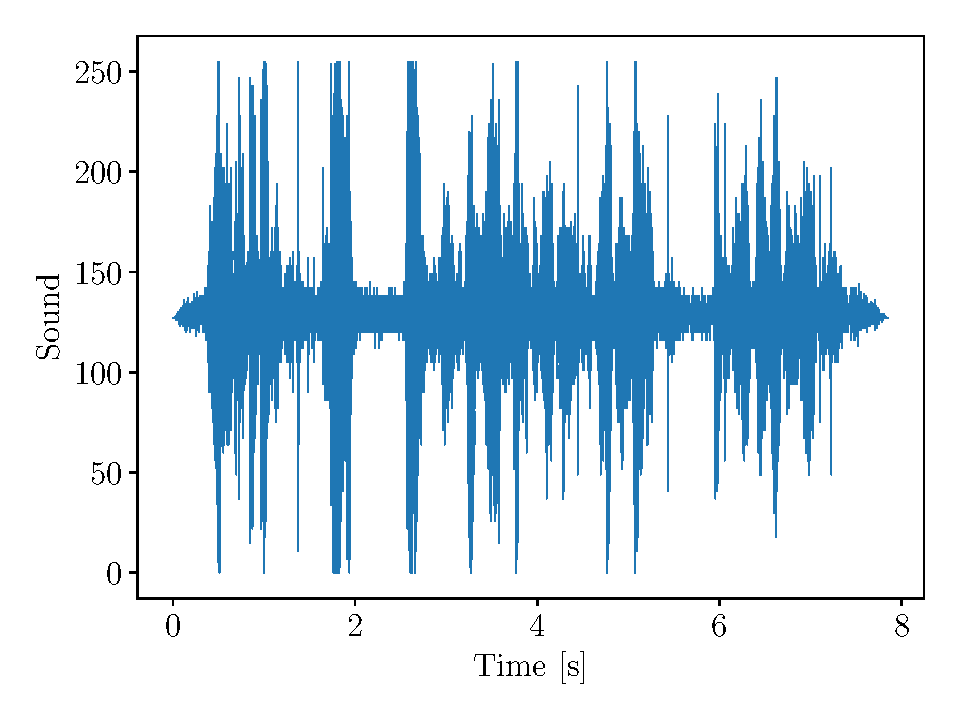
\includegraphics[width=0.75\textwidth]{resources/pdf/soundwave.pdf}
            \noskipcaption{Signal of \texttt{sound.wav}.}
            \label{fig:q15.soundwave}
        \end{figure}
        
        % Question 16
        
        \item The quantization of the sound signal is such that possible values are between 0 and 255. Therefore, 8 bits (a byte) must be used as it is the smallest number of bits for which all values of the signal can be encoded unequivocally. Indeed, one can represent $2^8 = 256$ different symbols using 8 bits.
        
        The encoding operation is therefore done by replacing the decimal values by their corresponding byte.
        
        % Question 17
        
        \item The channel has the effect of noising the signal. This effect has been simulated and the resulting noisy decoded signal is shown in Figure \ref{fig:q17.noisy.soundwave}.
        
        \begin{figure}[H]
            \centering
            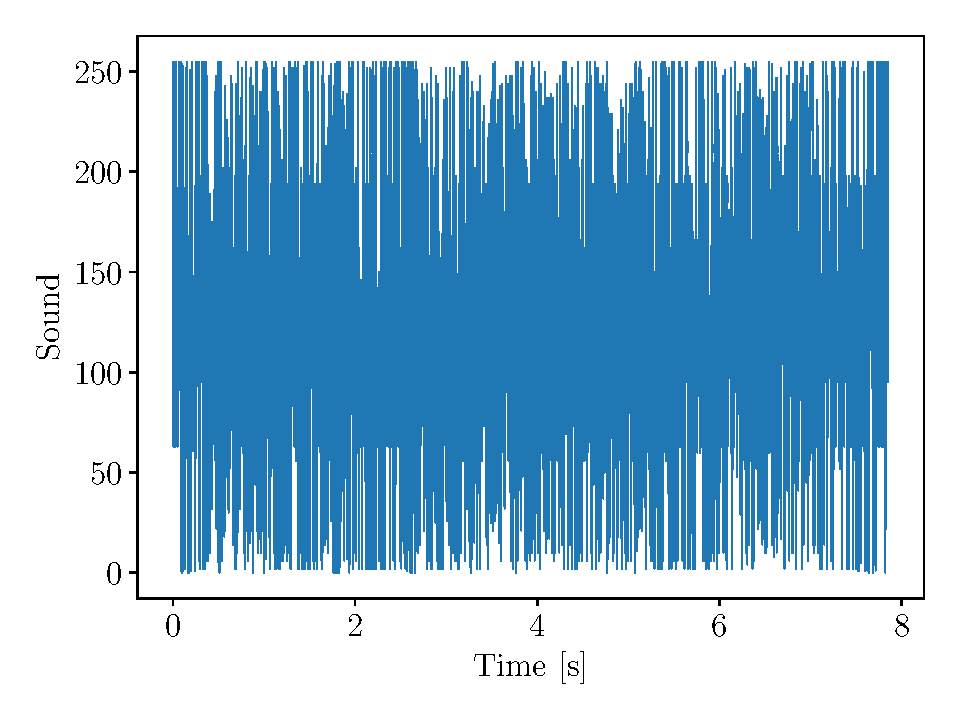
\includegraphics[width=0.75\textwidth]{resources/pdf/noisy_soundwave.pdf}
            \noskipcaption{Noisy decoded signal of \texttt{sound.wav}.}
            \label{fig:q17.noisy.soundwave}
        \end{figure}
        
        This corrupted version of the signal is still listenable but is spoiled by a very unpleasant background noise. This noise is clearly visible by comparing figures \ref{fig:q15.soundwave} and \ref{fig:q17.noisy.soundwave}. On the latter, the original signal shape is barely visible.
        
        % Question 18
        
        \item The requested function is defined in the class \texttt{Hamming} as \texttt{encode}.
        
        The original sound signal's length is \num{692520}. After being encoded with the defined function, its new length is \num{1211910}.
        
        % Question 19
        
        \item The effect of the channel has been simulated on the previously encoded binary sound signal with redundancy. The latter was then decoded and the result is presented in Figure \ref{fig:q19.noisy.decoded.soundwave}.
        
        \begin{figure}[H]
            \centering
            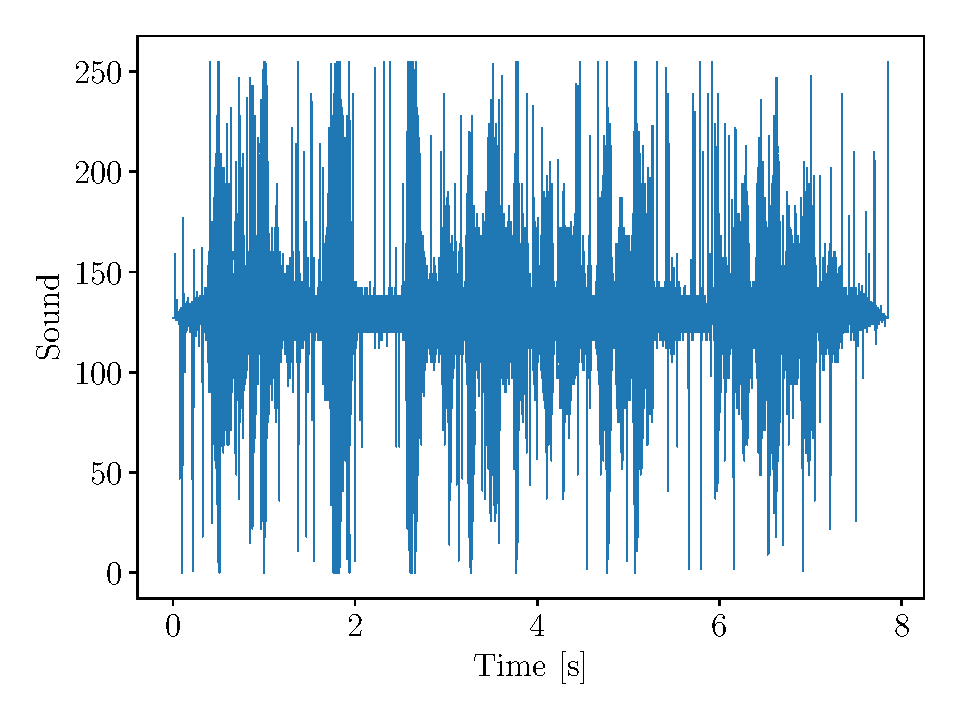
\includegraphics[width=0.75\textwidth]{resources/pdf/noisy_decoded_soundwave.pdf}
            \noskipcaption{Noisy decoded signal with redundancy of \texttt{sound.wav}.}
            \label{fig:q19.noisy.decoded.soundwave}
        \end{figure}
        
        A comparison between figures \ref{fig:q17.noisy.soundwave} and \ref{fig:q19.noisy.decoded.soundwave} shows that the decoded version of the signal with redundancy is much better than the decoded version of the original signal, yet a slight background noise is still audible.
        
        This result was expected as the redundant parity bits added by the Hamming (7,4) code allows to detect and correct part of the noise. Indeed, when a 7-bit codeword is received by the decoder, this one can compute the \emph{syndrome} of the codeword and decide whether or not the codeword as been altered and if so what bit. By construction, the syndrome, unless it is null, represents the index of the codeword's bit that is the more likely to be inverted. Inverting this bit will always produce a valid codeword that will be the original one most of the time, if the channel has a low probability of error. However, mistakes occur, that is why the decoded signal is not perfect.
        
        The procedure to decode the codewords is as stated above :
        \begin{itemize}
            \item The codeword's syndrome is computed using the parity-check matrix $H$;
            \item If not null, the corresponding bit is inverted to produce a valid codeword;
            \item The 4-bit word associated to the codeword is returned.
        \end{itemize}
        
        % Question 20
        
        \item To reduce the loss of information, additional parity bits, for example, could be used. This would make it possible to handle transmissions containing more errors. However, this requires the use of extra bits, \emph{i.e.} this will reduce the communication rate. As always, reducing the loss of information requires more resources.
        
        The communication rate could be improved by reducing the ratio of redundant bits over original bits. To do so, one could use an higher degree Hamming code such as $(15, 11)$ or $(255, 247)$\footnote{Our implementation actually allows to generate any Hamming code.}. Indeed, the communication rate of an Hamming $(2^r - 1, 2^r - r - 1)$ code is $$\frac{2^r - r - 1}{2^r - 1}$$ which tends to $1$ as $r$ increases. However, the higher $r$ the less the code is adapted to detect and correct errors.
    \end{enumerate}
    
    \newpage
    \printbibliography
    
\end{document}
